\documentclass{article}

% Includes preamble from standard file
% ==========================================================
%   GPR-20 MANUALS PREAMBLE
% ==========================================================

% ==========================================================
% Includes packages
\usepackage{parskip}
\usepackage{caption}
\usepackage{ltablex}
\usepackage{titlesec}
\usepackage{hyperref}
\usepackage{setspace}
\usepackage{graphicx}
\usepackage{xltabular}
\usepackage{csvsimple}
\usepackage{subcaption}
\usepackage{indentfirst}
\usepackage[utf8]{inputenc}
\usepackage[margin=1in]{geometry}
\usepackage[type={CC}, modifier={by-nc}, version={4.0}]{doclicense}
\usepackage{subfiles}
% ==========================================================

% ==========================================================
% PREAMBLE SETTINGS

% Allows use of X columns
\keepXColumns

% Sets double spacing
\doublespacing

% Sets paragraph indentation
\setlength{\parindent}{1em}

% Sets paragraph skip
\setlength{\parskip}{2em}
% ==========================================================


% Adds bibliography
\usepackage[style=numeric]{biblatex}
\bibliography{biblio.bib}


% Defines command to insert name
\newcommand{\GPRManualName}{Start Guide}

% ==========================================================
% DOCUMENT INFORMATION
\title{GPR-20: Start Guide}
\author{Grupo de Desminado Humanitario}
\date{July 2021}
% ==========================================================

\begin{document}

\subfile{front}

% INTRODUCTION
\newpage
\section{Introduction}
Landmines have caused 12,133 victims in Colombia as of January 2021 according to the Ministry of National Defense of the Country \cite{MINDEFENSA_STATISTICS}. From the 12,133 reported victims, 4,855 ($40.01\%$) are civilians while the remaining 7,278 are members of public forces \cite{MINDEFENSA_STATISTICS}. The Ministry's statistics report that 2,336 ($19.25\%$) of the victims perish from the accident, a value close to one (1) death out of five (5) accidents \cite{MINDEFENSA_STATISTICS}. Despite landmine removal efforts from the Government of Colombia and a sustained decrease through the last years, landmines accidents still occur. On hundred and forty one (141) accidents were reported in 2021 \cite{MINDEFENSA_STATISTICS}, indicating that both civilians and public forces are still in danger from landmines and unexploited ammunition.

The Universidad de Los Andes is a private research university located in Colombia that currently has an Humanitarian Demining Group as part its Department of Electric and Electronics Engineering, School of Engineering. The group promotes research, yet not exclusively, towards landmines removal and characterization. From January 2020 to March 2022, the Humanitarian Demining Group received a grant from both the National Academies of Science, Engineering and Medicine and the United States Agency for International Development (USAID) to gather data on landmines \cite{PEER_LANDMINES}. The project aims to help on the efforts of reducing the amount of victims from landmines in Colombia. As part of the project, the Group developed GPR-20, a portable robot designed to acquire data from different location in which landmines are found \cite{PEER_LANDMINES}. 

GPR-20 is a data acquisition robot used to develop new landmine detection models and algorithms. The robot uses the \textit{Ground Penetrating Radar} (GPR) technique to sample the ground in order to acquire signals that can be later used to detect landmines. The GPR is constructed using a \textit{Vector Network Analyzer} (VNA) and two PowerLOG 70180 antennae with a bandwidth of up to 5.4 GHz. The antennae are moved within the sampling area by the means of a Cartesian robot constructed using 3D printing parts. An user interface is also present in the robot to allow interaction.

An user should be able to understand the basics from the operational principles, structure and purpose of the robot by reading this document. Nevertheless further documentation is referred depending on the role of the user. Two roles are assumed from a reader: user and developer. The user is the person that will only interact with the GPR-20 to use it while the developer will interact with the robot to improve its design and performance. Further documentation for an user is a set of operational manuals for surveys. On the other hand, documentation for developers is a set of detailed documentation and guidelines for development processes.

This document consists of three main sections: an introduction of the GPR-20 robot, a reference of the robot documentation, and the repositories of the project. The introduction presents a general overview of the robot as it introduces the operation principles and its main subsystems. The reference section intends to serve as the starting point from which the reader could seek information of his/her interest. The reader should keep in mind that this guide is a start guide in which only a general information is presented. Finally, the last section provides the links to the project repositories. Repositories include both the documents and the required files for the robot to work.


\newpage
\section{GPR-20 Overview}
This section presents a general overview of the GPR-20 robot. In first place, a brief review of the operational principle is introduced i.e. the \textit{Ground Penetrating Radar}. Then an overview of the robot itself is presented. This overview consists of the mechanical structure, data acquisition and electronics. A reader should be able to get a basic understanding of how the GPR-20 robot works by reading this section.

GPR-20 is a robot whose purpose is to acquire data from deactivated minefields. Data acquired using the robot will be available to researchers around the world interested in developing new detection algorithms for landmines that pose a risk for rural communities. GPR-20 design itself will be also available for groups and institutions that might want to replicate or further develop the system. In general terms, GPR-20 objective is to allow a broader scientific community to take part into landmine removal. 

\begin{figure}[ht]
    \centering
    \vspace{0.5cm}
    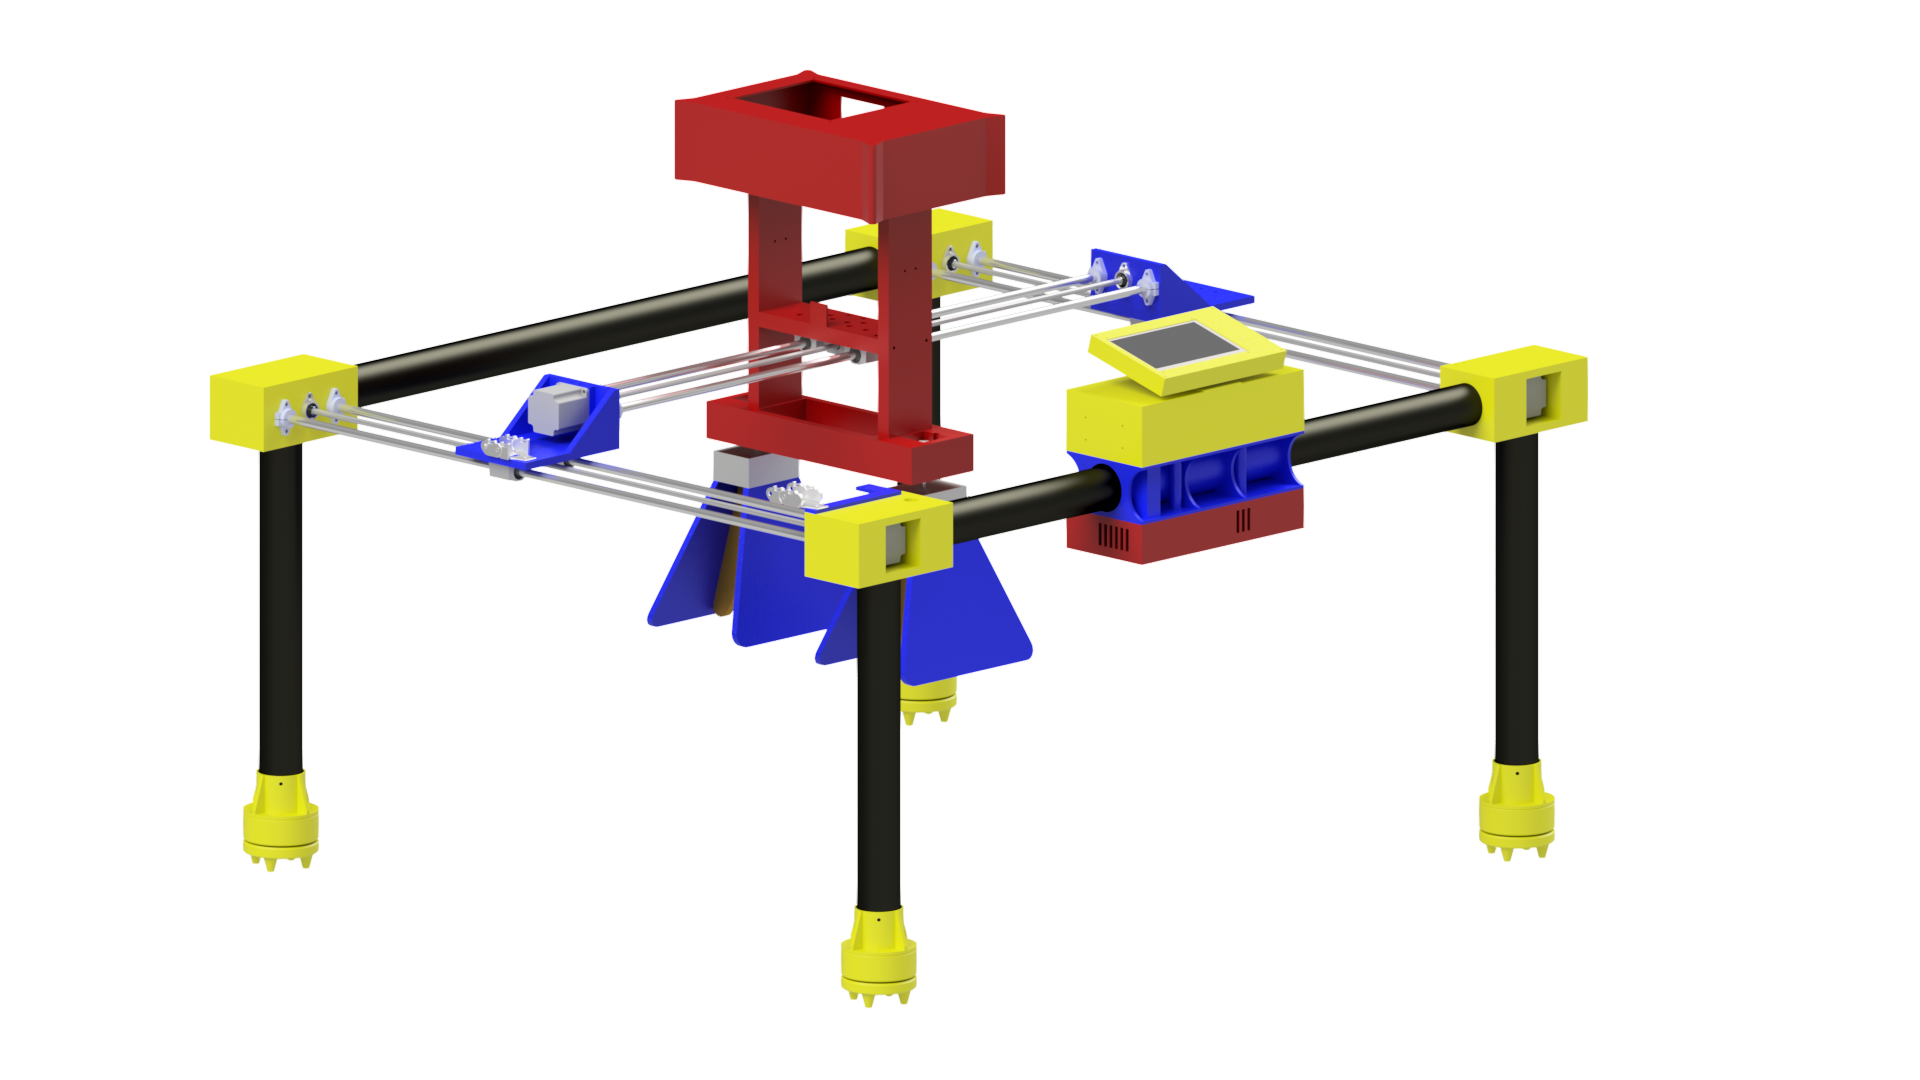
\includegraphics[width=0.85\textwidth]{images/full_mkII.png}
    \caption{GPR-20 render.}
    \label{fig:gpr-gpr20}
\end{figure}

Figure \ref{fig:gpr-gpr20} presents a render of the GPR-20 robot. The robot consists of a mechanical structure that holds a Cartesian robotic arm used to moves a positioner. The positioner is the mechanical element that moves within the sampling area and holds both the antennae and the VNA. There is another element on one of the robot sides that has a touchscreen from which the robot can be controlled. This element also stores the electronics and power systems. The robot itself is powered from an external AC source and might use an external laptop to process and analyze data as it is sampled. 

\subsection{Operation Principles}
GPR-20 operation principle is the \textit{Ground Penetrating Radar} (GPR) method. GPR is a method that uses radio waves to acquire data from the soil. There are two main methods for acquiring data using a GPR: trough reflected waves from subsurface features or transillumination of a volume. GPR-20 relies on the reflections method as is shown on figure \ref{fig:gpr-principle}. The method of reflections consists of setting up a receiver and a transmitter in a fixed geometry that is later moved to detect reflections from underground elements \cite{GPR_JOL}. 

\begin{figure}[ht]
    \centering
    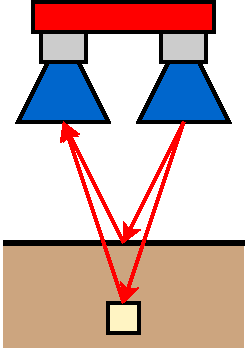
\includegraphics[width=0.35\textwidth]{images/GPR_principles.pdf}
    \caption{Depiction of the GPR method used on the GPR-20 robot.}
    \label{fig:gpr-principle}
\end{figure}

Data acquired from the GPR consists of a set of frequency-domain values equally distributed within the bandwidth. The bandwidth used for surveys is 5.4GHz starting from 600MHz in which the amount of data points range from 256 to 4000 points. Frequency-domain data can be transformed into time-domain signals that can be interpreted as A-Scans. A-Scans can be then merged into B-Scans and C-Scans which allows visualization and analysis of two-dimensional and three-dimensional data respectively. Figure \ref{fig:gpr-scans} presents an A-Scan, B-Scan and C-Scan acquired using data acquired from a GPR. Acquisition on the GPR-20 robot is done on surveys, which consist of sampling the ground on a set of predefined spatial points. These predefined points add up to sample data from a straight line or a rectangular area. GPR-20 is able to acquire data from an area size up to 800$\times$800 square millimeters (mm\textsuperscript{2}).

\begin{figure}
    \centering
    \begin{subfigure}[b]{0.4\textwidth}
        \centering
        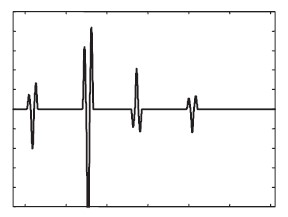
\includegraphics[width=\textwidth]{images/A_Scan_sample.jpg}
        \caption{A-Scan signal acquired from a GPR.}
        \label{fig:gpr-a-scan}
    \end{subfigure}
    \hfill
    \begin{subfigure}[b]{0.4\textwidth}
        \centering
        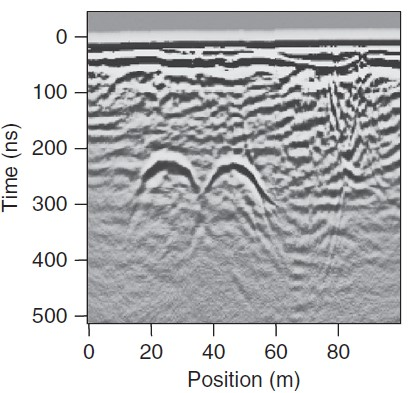
\includegraphics[width=\textwidth]{images/B_Scan_sample.jpg}
        \caption{B-Scan signal acquired from a GPR.}
        \label{fig:gpr-b-scan}
    \end{subfigure}
    \vfill
    \begin{subfigure}[b]{0.6\textwidth}
        \centering
        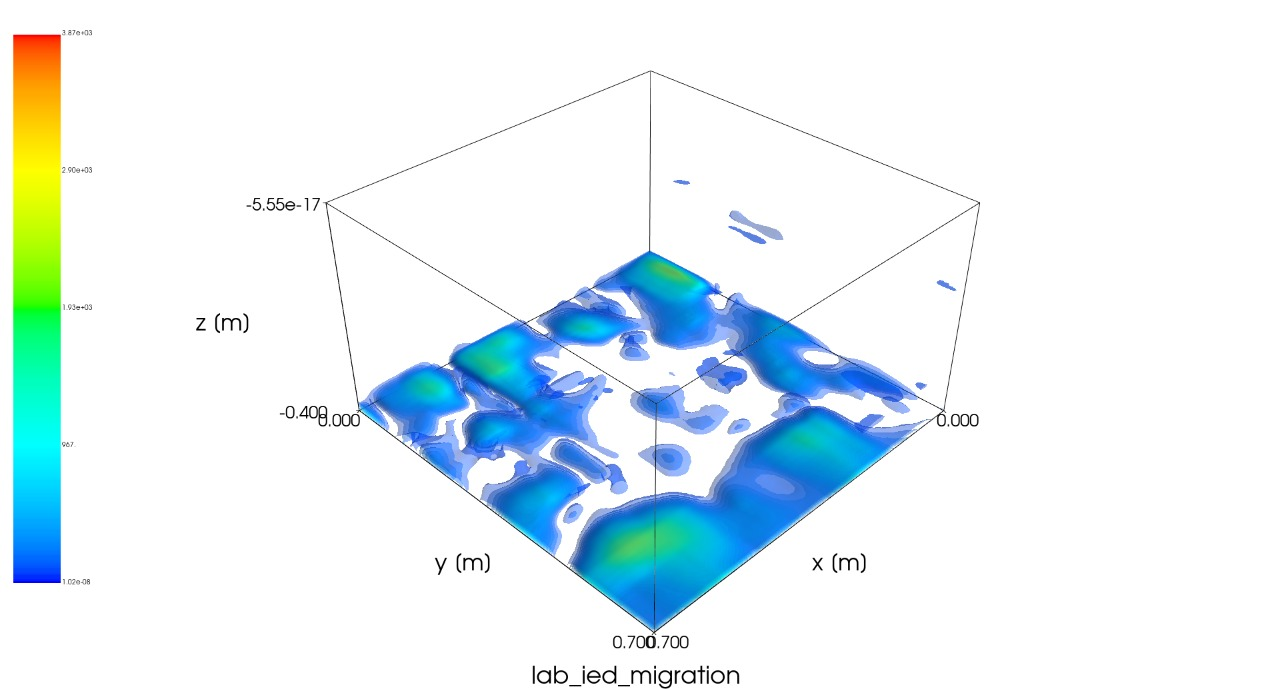
\includegraphics[width=\textwidth]{images/C_Scan_sample.jpeg}
        \caption{C-Scan signal acquired from a GPR.}
        \label{fig:gpr-c-scan}
    \end{subfigure}
    \caption{Different data representations using data acquired from a GPR.}
    \label{fig:gpr-scans}
\end{figure}


\subsection{Mechanical Structure}
GPR-20 works over a structure that supports the data acquisition, electric and mechanical elements required to use the robot. The structure in which the robot relies is built from 3D printed parts, PVC tubing and miscellaneous elements like screws and nuts. This scheme allows for quick prototyping and ease of replication. GPR-20 is shown on figure \ref{fig:gpr-gpr20} in which the structure can be identified. 


\subsection{Data Acquisition}
GPR-20 acquires data by using the GPR method using two antennae and a VNA. Nevertheless a GPR data pipeline requires processing units and software that allows for coordinating data acquisition and processing. Data acquisition using the GPR-20 robot requires coordination between the Cartesian arm, the GPR and processing units. Figure \ref{fig:gpr-data} presents the data acquisition and analysis pipeline.

\begin{figure}[h]
    \centering
    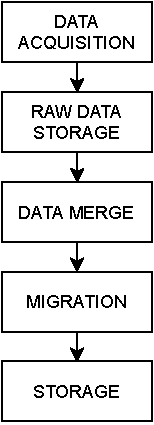
\includegraphics[width=0.2\textwidth]{images/data_pipeline.pdf}
    \caption{Data pipeline for the GPR-20 robot.}
    \label{fig:gpr-data}
\end{figure}

The data acquisition process begins with the sampling of the ground with the antennae and the VNA. The results of each sampling point are stored as raw data. After the survey is finished, data is merged into a single file that allows analysis of a 3D sampled volume. To improve data quality and value, a migration process is applied to the data. Finally, the migrated data is stored as the result of the survey process.


\subsection{Electronics}
Electronics from the GPR-20 robot can be divided into two subsystems: power and data. Power subsystem is in charge of supplying electrical energy into every robot component. Data subsystem is the organization and interconnection of electronic components that allow for data acquisition and processing. 

\newpage
\section{Documentation}
This section presents the further documentation that the reader might be interested in. Two roles of readers can be identified: an user or a developer. The user is the person that will use the robot to acquire data without enhancing the robot features or improving its performance. The developer is the person that will use the robot to add new features or improve the existing ones. Links to document repositories are presented in the third section of this document. Each document is intended to be used by one of the two roles of readers described before.

\subsection{Start Guide}
This document serves as the start guide for the GPR-20 robot. It presents a general overview of the robot and references to further documentation. This document also includes links to different project repositories regarding documentation and robot files. This is the only document that should be read by both roles of reader. 

\subsection{Development History}
The development history document introduces the process of creating the GPR-20 robot. The reader should be able to understand the context in which the robot was developed, why it was developed and how the processes influenced both the group and its people. This document is optional for both roles of readers and it is intended for informational purposes only.

\subsection{Field Setup Manual}
The field setup manual contains specific instruction on how setup the robot to perform a field survey. Setup of the GPR-20 robot starts by assembling the robot according to field requirements. Then instructions of how to connect data and electrical signals of the robot are defined. An inverse process including disconnection and disassembly of the robot is also presented in the document. This document is intended to be read by an user.

\subsection{Field Use Manual}
The field use manual presents the required steps to perform a survey and acquire data with the robot. This document serves as a continuation of the field setup manual as it is limited to the interactions of the user with the robot's interface. By reading both the field setup manual and the field use manual it is expected that an user should be able to move the robot into the field, acquire data and move it back into storage. This is document expected to be read by an user.

\subsection{Basic Assembly Manual}
This document contains the required instructions to build and assembly the robot. This document main intention is to allow for replication of the project. This is achieved by presenting detailed steps and processes that allows a third-party group or institution to build their own robot. This document is intended to be read by an user, but a developer might be interested on it.

\subsection{Software Guide}
This is a guide that introduces and presents the software used on the GPR-20 robot. An introduction of the used tools and frameworks, software structure and organization is presented in first place. Then detailed information of each software module of the robot is presented and discussed. Finally, considerations on software development as coding style and conventions are presented. This document is expected to be read by a developer.

\subsection{Mechanical Structure Guide}
This document presents information related to the mechanical structure of the robot. An introduction on the mechanical structure is presented in first place. Detailed information on each components of the structure is then presented. Finally, guidelines for future development are discussed. This document is expected to be read by a developer.

\subsection{Data Acquisition Guide}
The data acquisition guide presents information regarding the data acquisition and analysis. In first place, it contains the theoretical foundations of the data acquisition and processing. Then, aspects on how the data acquisition and analysis was implemented are presented. Finally, options for further development are introduced. This document is expected to be read by a developer.

\subsection{Electronics and Power Guide}
Presents the information on electronics and power systems of the GPR-20 robot. This documents presents detailed information on the organization and design of both the power and electronics systems. The scheme used on the robot is presented and considerations for future modifications. This document is expected to be read by a developer.

\subsection{Test Report}
Presents the testing procedures and results for the GPR-20 robot. This document introduces the testing procedures that were designed to validate the GPR-20 robot operation regarding the mechanical structure, power and electronic systems, and software. Results are presented to effectively validate that the robot operates as intended. This document is expected to be read by both a developer and an user.

\newpage
\section{Repositories}
Documents and project files are stored in public repositories in order to be accessed by the community. Repositories include the necessary additional files for fulfilling the roles of both a developer and an user. The repositories contain files for both the user and developer roles. User files in repositories contain files that are ready for use while developer files contain the editable source files. Repositories are also divided depending on its focus: documents, mechanical structure, power and electronic systems, and software. Document repositories are in table \ref{tab:docs_repositories}, mechanical structure repositories are presented in table \ref{tab:mechanical_repositories}, power and electronics repositories are presented in table \ref{tab:power_repositories}, and software repositories are presented in table \ref{tab:software_repositories}.

\begin{singlespace}
    \begin{xltabular}{\textwidth}{|p{4cm}|X|}
    
    \hline \multicolumn{2}{|c|}{\textbf{Documents}} \\ \hline
    \textbf{Name} & \textbf{Link} \\ \hline
    \endhead
    
    \hline \multicolumn{2}{|c|}{\textbf{Documents}} \\ \hline
    \textbf{Name} & \textbf{Link} \\ \hline
    \endfirsthead
    
    \hline \multicolumn{2}{|c|}{\textit{Continues in next page.}}
    \endfoot
    
    \caption{Document repositories for the GPR-20 robot.} \label{tab:docs_repositories}
    \endlastfoot
    
    Start Guide & \url{https://github.com/gdh-uniandes/gpr20_start_guide} \\ \hline
    Development History & \url{https://github.com/gdh-uniandes/gpr20_development_history} \\ \hline
    Field Setup Manual & \url{https://github.com/gdh-uniandes/gpr20_field_setup_manual} \\ \hline
    Basic Assembly Manual & \url{https://github.com/gdh-uniandes/gpr20_basic_assembly_manual} \\ \hline
    Software Guide & \url{https://github.com/gdh-uniandes/gpr20_software_guide} \\ \hline
    Mechanical Structure Guide & \url{https://github.com/gdh-uniandes/gpr20_mechanical_guide} \\ \hline
    Data Acquisition Guide & \url{https://github.com/gdh-uniandes/gpr20_data_acquisition_guide} \\ \hline
    Electronics and Power Systems Guide & \url{https://github.com/gdh-uniandes/gpr20_electronics_power_guide} \\ \hline
    Test Report & \url{https://github.com/gdh-uniandes/gpr20_test_report} \\ \hline
    \end{xltabular}
\end{singlespace}

\begin{singlespace}
    \begin{xltabular}{\textwidth}{|p{4cm}|X|}
    
    \hline \multicolumn{2}{|c|}{\textbf{Mechanical Structure}} \\ \hline
    \textbf{Name} & \textbf{Link} \\ \hline
    \endhead
    
    \hline \multicolumn{2}{|c|}{\textbf{Mechanical Structure}} \\ \hline
    \textbf{Name} & \textbf{Link} \\ \hline
    \endfirsthead
    
    \hline \multicolumn{2}{|c|}{\textit{Continues in next page.}}
    \endfoot
    
    \caption{Mechanical structure repositories for the GPR-20 robot.} \label{tab:mechanical_repositories}
    \endlastfoot
    
    Ground Support & \url{https://github.com/gdh-uniandes/gpr20_ground_support} \\ \hline
    Cartesian Arm & \url{https://github.com/gdh-uniandes/gpr20_cartesian_arm} \\ \hline
    VNA Holder & \url{https://github.com/gdh-uniandes/gpr20_vna_holder} \\ \hline
    Electronics Box & \url{https://github.com/gdh-uniandes/gpr20_electronics_box} \\ \hline
    
    \end{xltabular}
\end{singlespace}

\begin{singlespace}
    \begin{xltabular}{\textwidth}{|p{4cm}|X|}
    
    \hline \multicolumn{2}{|c|}{\textbf{Power and Electronic Systems}} \\ \hline
    \textbf{Name} & \textbf{Link} \\ \hline
    \endhead
    
    \hline \multicolumn{2}{|c|}{\textbf{Power and Electronic Systems}} \\ \hline
    \textbf{Name} & \textbf{Link} \\ \hline
    \endfirsthead
    
    \hline \multicolumn{2}{|c|}{\textit{Continues in next page.}}
    \endfoot
    
    \caption{Power and Electronic Systems repositories for the GPR-20 robot.} \label{tab:power_repositories}
    \endlastfoot
    
    GPR-20 PCB & \url{https://github.com/gdh-uniandes/gpr20_pcb} \\ \hline
    
    \end{xltabular}
\end{singlespace}

\begin{singlespace}
    \begin{xltabular}{\textwidth}{|p{4cm}|X|}
    
    \hline \multicolumn{2}{|c|}{\textbf{Software}} \\ \hline
    \textbf{Name} & \textbf{Link} \\ \hline
    \endhead
    
    \hline \multicolumn{2}{|c|}{\textbf{Software}} \\ \hline
    \textbf{Name} & \textbf{Link} \\ \hline
    \endfirsthead
    
    \hline \multicolumn{2}{|c|}{\textit{Continues in next page.}}
    \endfoot
    
    \caption{Software repositories for the GPR-20 robot.} \label{tab:software_repositories}
    \endlastfoot
    
    Axis Driver & \url{https://github.com/gdh-uniandes/gpr20_axis_driver} \\ \hline
    Height Sensor & \url{https://github.com/gdh-uniandes/gpr20_height_sensor} \\ \hline
    VNA Acquisition & \url{https://github.com/gdh-uniandes/gpr20_vna_acquisition} \\ \hline
    VNA Processing & \url{https://github.com/gdh-uniandes/gpr20_vna_processing} \\ \hline
    Main Control & \url{https://github.com/gdh-uniandes/gpr20_main_control} \\ \hline
    User Interface & \url{https://github.com/gdh-uniandes/gpr20_user_interface} \\ \hline
    
    \end{xltabular}
\end{singlespace}

\newpage
\printbibliography


\end{document}
